\chapter{Synthèse}
\section{Synthèse FRF}

\subsection{Principe}
% méthode hybride ici. mélange mesures et théorie
\paragraph*{} 

Le principe de la synthèse dans le domaine fréquentiel est relativement simple.
Il s'agit de calculer ou de mesurer des fonctions de transfert
(\textit{Frequency Response Function}) nous permettant de relier une force
appliquée au point d'excitation de la corde à un déplacement au niveau du
chevalet, de la table d'harmonie de la guitare, ou d'un autre instrument comme le ukulélé. On parle de méthode hybride puisqu'elle conjugue modèles théoriques et mesures sur instruments. Le premier élément nécessaire est l'admittance au chevalet, qui peut s'exprimer grâce à l'admittance des cordes et celle du corps au niveau du chevalet (par corps, il faut comprendre la table d'harmonie et la caisse de la guitare), par l'équation \ref{eq:eq_frf_1}.

Cette admittance totale au niveau du chevalet nous fournit la vitesse de
celui-ci en fonction d'une force qui y serait appliquée.

Le second élément nécessaire est la fonction de transfert $H$ reliant un
déplacement de la corde à un déplacement au niveau du chevalet. En multipliant cette fonction avec $Y_{total}$, on obtient la FRF fournissant le déplacement $\delta_{excitation}$ en fonction de la force $F_{chevalet}$. Le système étant supposé linéaire, le principe de réciprocité de Betty s'applique et cette fonction de transfert fournit aussi le déplacement $\delta_{chevalet}$ en fonction de la force $F_{excitation}$ (équation \ref{eq:eq_frf_2}).


\subsection{Mise en place}
% implémentation
% H, Z, Ytotal
\subsubsection{Formulations théoriques}
L'article de Woodhouse à notre disposition nous permet d'écrire l'impédance
de la corde au chevalet $Z_{corde}$, ainsi que la fonction de transfert
unitaire $H$ à partir de la connaissance des caractéristiques de la corde :
masse linéique, tension, coefficients d'amortissement, raideur de flexion (équations \ref{eq:eq_frf_4} et \ref{eq:eq_frf_5}). Ces fonctions de transfert sont dépendantes de l'écriture des modes de corde et le modèle de leur amortissement choisi par Woodhouse est présenté à l'équation \ref{eq:eq_frf_4}.

\subsubsection{Mesures sur la guitare}
Les mesures sur les instruments fournissent une estimation de $Y_{corps}$ et de $Y_{total}$.

La première approche est d'utiliser uniquement $Y_{total}$ mesurée en
excitant au marteau d'impact un point proche du chevalet et en mesurant son accélération selon l'axe normal et l'axe transverse par rapport à la table
d'harmonie. La corde que l'on souhait synthétiser est libre de vibrer
alors que les autres sont étouffées. En réalité, nous mesurons l'inertance,
ce qui doit ajouter une seconde intégration à l'équation \ref{eq:eq_frf_2}.

La seconde approche est de n'utiliser que la mesure de $Y_{corps}$ .
L'admittance de la corde $Y_{corde}$ au chevalet utilise les formulations théoriques de l'article (équation~\ref{eq:eq_frf_4}) pour obtenir $Y_{total}$.

\subsubsection{Implémentation}
Les FRF issues des mesures temporelles sont calculées avec un très grand nombre de points pour que le signal final dure plusieurs secondes. L'obtention du son est en effet réalisée par FFT inverse, ce qui nous impose d'écrire la symétrie hermitienne pour notre fonction de transfert pour assurer que le signal synthétisé est bien réel.

L'intégration de l'équation~\ref{eq:eq_frf_2} fournit des valeurs en basses fréquences divergentes en zéro. Pour compenser cela nous intégrons dans le domaine fréquentiel en imposant des valeurs très faibles de la FRF en-dessous de
\( \si{50\Hz} \) (notre note la plus basse était un Mi grave de
\( \si{83\Hz} \)).

Enfin, nous convoluons ce signal avec une ou plusieurs impulsions consécutives pour adoucir le son par un filtrage passe-bas et modéliser une force qui dure dans le temps.

\subsection{Résultats}
%

Utiliser $Y_{total}$ mesuré ne fournit pas de résultats convaincants. Les sons synthétisés ne correspondent pas à ceux d'une guitare. Woodhouse suggère en effet d'effectuer la séparation de cette grandeur, ce que nous avons choisi de faire exclusivement.

Toutes les cordes à vide de la guitare sont synthétisées, avec comme excitation une force ponctuelle et une force qui dure dans le temps, ceci pour chaque mesure d'amittance à notre disposition. La partie théorique de cette synthèse utilise 40 modes de cordes, et les sons obtenus durent 11 secondes. On reconnait clairement un son de guitare à l'écoute. Voici une des fonctions de transfert obtenues de notre système :

\begin{figure}[h]
\centering
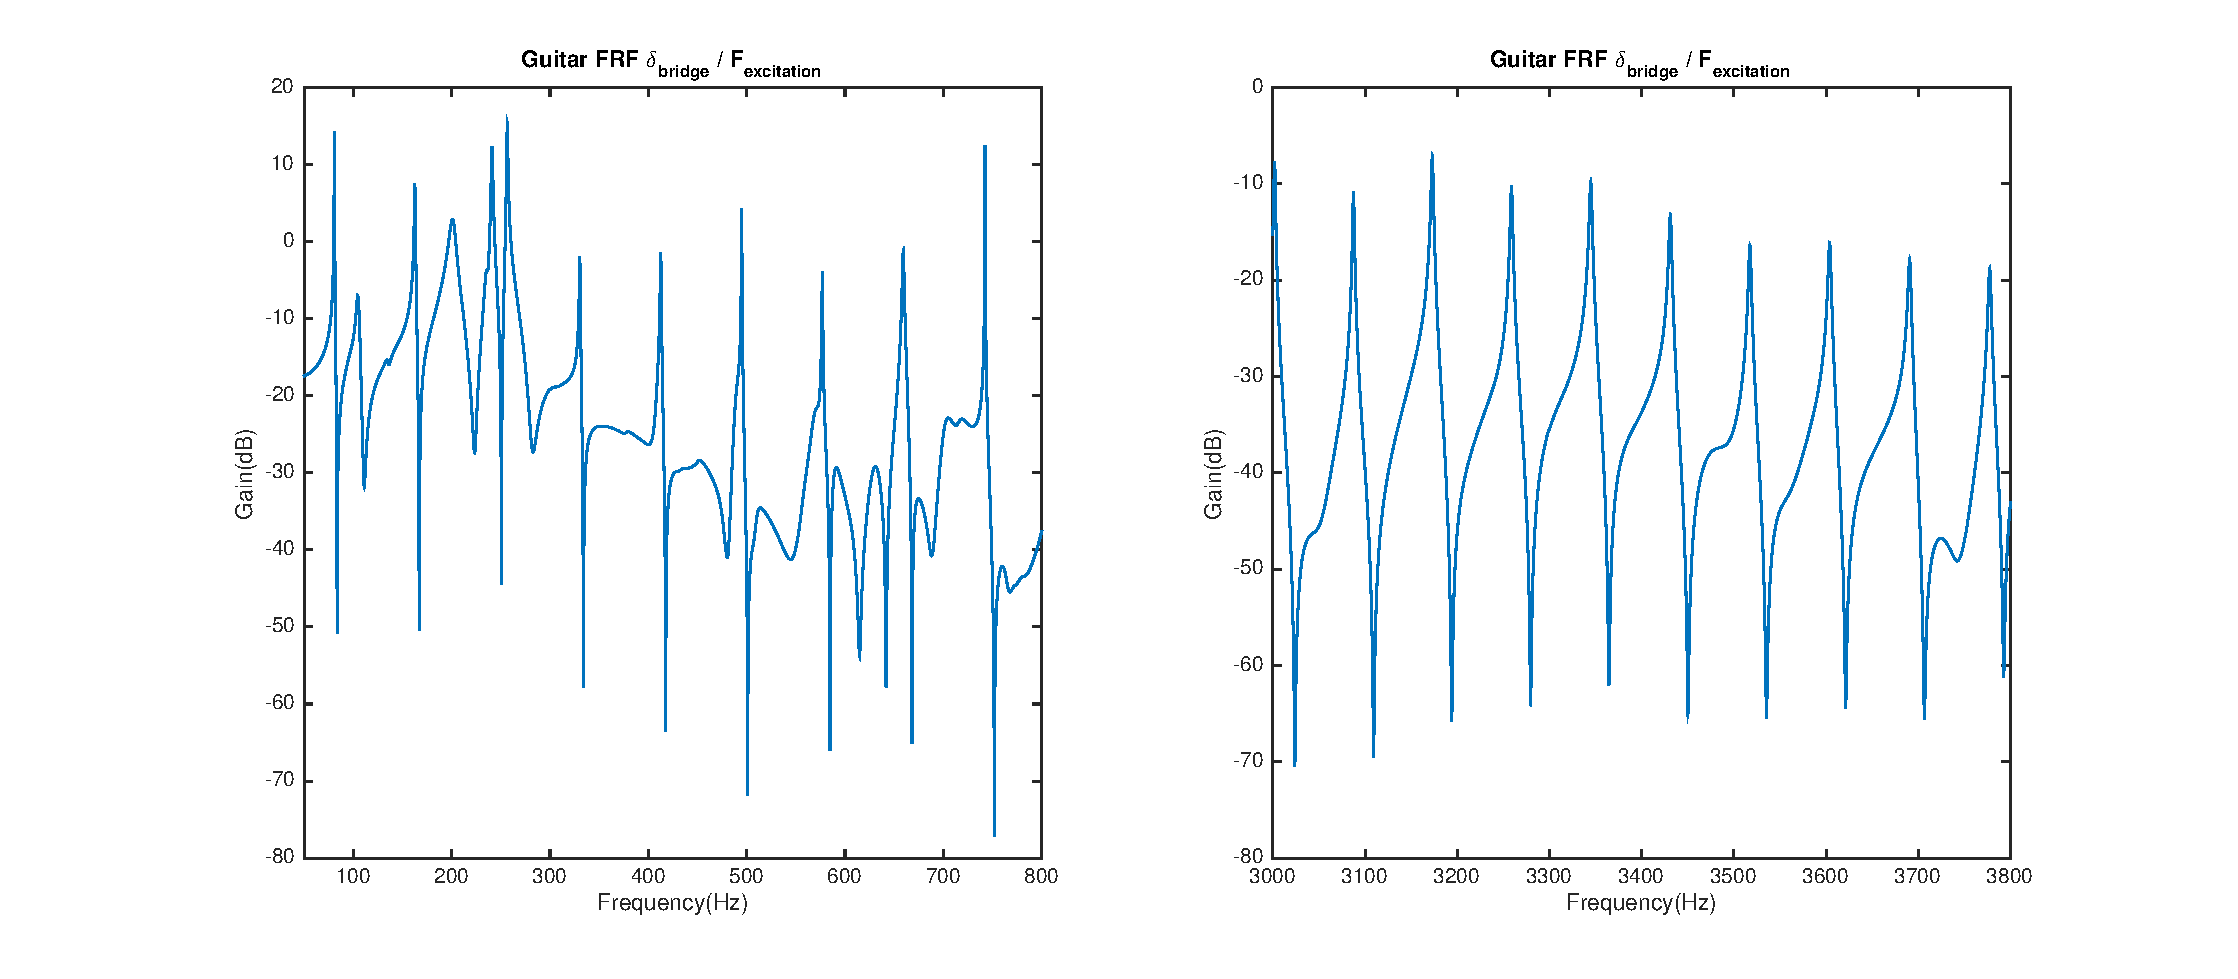
\includegraphics[width=\linewidth]{figures/FRF_E2.eps}
\caption{Admittance de la synthèse hybride}
\label{fig:frf_fig_1}
\end{figure}

Plusieurs précisions ont du être apportés pour améliorer l'algorithme et le
son. En effet, ce système comporte plusieurs limitations : l'admittance
$Y_{corps}$ est affectée par la présence de cordes même atténuées. Cet effet est difficilement écarté puisqu'ôter les cordes de l'instrument modifie la masse au niveau du chevalet. Aussi, nous n'avons pas mesuré les caractéristiques des cordes de la guitare à notre disposition mais nous sommes basés sur des valeurs fournies par Woodhouse, qui peuvent ne pas correspondre à notre instrument.\\


%
%
% $c$ pour chevalet, $e$ pour excitation.
% $$\frac{1}{Y_{tot}} = \frac{1}{Y_{corps}} + \frac{1}{Y_{corde}}$$
%$$F_c \times Y_{tot} = v_c$$
%$$v_c \times \tilde{H} = v_e$$
%$$\frac{v_e}{j\omega} = \delta_e$$
%par théorème de réciprocité de Betty : 
%$$\frac{\delta_c}{F_e} = \frac{\delta_e}{F_c} = \frac{Y_{tot}\tilde{H}}{j\omega}$$
%
%


\section{Synthèse modale}

\paragraph{}
  On présente dans cette partie le processus d'analyse/synthèse modale hybride
appliqué dans le cadre du projet. Ce processus est basé sur les principes
suivants : les paramètres physiques découplés de corde et de guitare sont
posés, pour la corde via un modèle théorique, pour le corps en appliquant
\textsc{esprit} sur les mesures d'admittance effectuées et en remontant aux
paramètres physiques du système.
  Ensuite, le système d'équations différentielles à \( N \) modes du système
couplé est posé et on résout ce système pour en extraire les déformées modales
et les fréquences propres du système couplé. Enfin, en fixant des
conditions initiales, on peut synthétiser le son de la corde couplée au
chevalet.

  L'intérêt de cette méthode face à la méthode par FRF est la possibilité
d'accéder directement à des paramètres physiques pertinents du problème et
d'ainsi pouvoir les modifier pour écouter leur effet sur le son synthétisé.
  En outre, la résolution du système du premier ordre avec matrice
d'amortissement retourne des modes complexes et prend donc naturellement en
compte l'amortissement de chaque mode couplé et évite l'effet de
"\emph{veering}" décrit par Woodhouse.

\subsection{Paramètres physiques}

\paragraph{}
  Par souci de concision, on ne présente pas dans ce rapport le détail des
matrices développées dans l'article de Woodhouse, mais seulement la façon dont
les paramètres physiques pertinents peuvent être extraits ou fixés.

\subsubsection{Corde}
  \paragraph{}
  
  La corde suit un modèle théorique basé sur sa longueur \( L \), sa tension
\( T \), sa raideur de torsion \( B \) et sa masse linéique \( \rho{} \).
  On choisit ensuite le nombre de modes de corde désiré.
  Pour une corde de Mi grave (\( E2 \)), dont la fréquence fondamentale est
de \( \si{82.4 \hertz}\), le \( 39 \)ème harmonique aura une fréquence (modulo 
inharmonicité) proche de \( \si{3214\hertz} \), c'est la valeur maximale que
l'on fixe.

  Concernant les conditions aux limites, la corde est supposée fixe-fixe
en isolation et le couplage est ensuite réalisé au niveau du chevalet à l'aide
d'un mode de contrainte rigide qui permet d'inclure les vibrations du corps.

\subsubsection{Corps}

  \paragraph{}
  Les paramètres physiques du corps sont extraits par analyse modale via ESPRIT.
Attendu que la densité modale devient très élevée au-delà de \( \si{1500\Hz} \),
et sachant que la première fréquence de résonance du corps est de l'ordre de
\( \si{100\Hz} \), on cherche des fréquences de résonance de corps dans
l'intervalle de \( \si{90\Hz} \) à \( \si{1500\Hz} \).
On ne considère donc que \( 15 \) modes de corps, dans l'ordre des observations
sur cette plage de fréquence.

Woodhouse pose dans les hautes fréquences un modèle de distribution modale
statistique qui n'est pas considéré ici.

%   Une fois les fréquences propres et les amortissements du corps isolé
% extraits, on en déduit les paramètres physiques du corps au niveau du
% chevalet, modélisé comme un ensemble unidimensionnel de systèmes masse-ressorts
% à \( N_b \) modes, d'admittance :
%   \[ Y(\omega) = \sum_{k=1}^{N_b} \frac{j\omega{}}
%     {m_k(\omega_k^2 + 2 j \omega{} \omega{}_k \xi{}_k - \omega{}^2)} \]
    
% Pour ce faire, on définit pour chaque mode calculé une masse effective
% \( m_k \) et une raideur effective \( s_k \) ainsi définies :

\paragraph*{}

Parmi les paramètres physiques utilisés par Woodhouse, les masses modales
posent un léger problème : Woodhouse ne fournit qu'une expression qui suppose
de connaître les amplitudes au niveau du chevalet des déformées modales
relatives à chaque mode de corps, valeurs requérant une analyse modale
complète du système.
  
  On remplace ce calcul par une valeur proposée par~\textcite{pate14:phd}.
  Les masses modales sont obtenues par inversion locale autour de
\( \omega = \omega_k \) de l'expression de l'admittance et
valent \[ m_k = \frac{1}{2 |Y(\omega_k)| \omega{}_k \xi{}_k} \] une valeur plus
simple à calculer que celle proposée par Woodhouse.

\subsubsection{Couplage par équations différentielles matricielles}

  \paragraph*{}
  L'étape suivante est la définition --classique -- du système d'équations
différentielles cou\-plées :
\[ M \ddot{\bm{q}} + C \dot{\bm{q}} + K \bm{q} = \bm{F} \]

  Les valeurs des matrices \( M \) et \( K \), respectivement de masse et de
raideur, sont obtenues dans l'article de Woodhouse par une analyse énergétique
du système et une inversion des résultats obtenus (une sorte de fitting modal).

  L'amortissement est supposé (hypothèse simplificatrice choisie par Woodhouse)
visqueux (i.e. proportionnel pour chaque mode découplé à sa vitesse) et la
matrice d'amortissement \( C \) est donc diagonale dans la base des
modes découplés.

Notons que, bien que très classique et naturelle, la conversion en système
d'équations différentielles du premier ordre est entachée d'erreur dans
l'article de Woodhouse, qui intervertit les matrices \( C \) et \( K \), ce
qui a été la cause de pas mal de tracas\dots

\subsection{Somme modale}

  La synthèse modale est effectuée selon des formules décrites
dans le livre de~\textcite{newland}, qui traduisent une sommation des modes
pondérée par les amplitudes issues des conditions initiales.

  La condition initiale choisie est actuellement un déplacement triangulaire
de la corde, avec prise en compte d'une largeur de doigt (d'un \( \si{\cm} \))
qui opère comme un filtre passe-bas.

\subsection{Statut de l'implémentation et observation de résultats}

Les valeurs requises ayant été obtenues comme décrit dans le chapitre suivant,
l'implémentation de la synthèse modale hybride est pleinement fonctionnelle
et efficace (moins de 10 secondes de calcul au total, calcul des paramètres
inclus, pour synthétiser 30 secondes de signal) et pourrait donc opérer en
temps réel.

Les résultats de la synthèse sont comparés avec les valeurs mesurées dans une
partie à venir.

On propose en Figure~\ref{fig:synth:modal_synth} la visualisation du résultat
de la synthèse du son de la corde \( E2 \) avec prise en compte d'une largeur
de doigt, à \( \si{11\cm} \) du chevalet et un point d'écoute à
\( \si{26\cm} \) du chevalet.
On utilise \( 40 \) modes de corde et \( 15 \) modes de corps.
On observe bien une enveloppe temporelle en exponentielle décroissante lente
(décroissance de l'ordre de 5 à 10 secondes) et une répartition harmonique
des fréquences propres, qui s'arrête autour de
\( f_{max, graph} = \si{3300\Hz} \), comme attendu d'après le nombre de modes
fixé.

\begin{table}[hpbt]
\centering
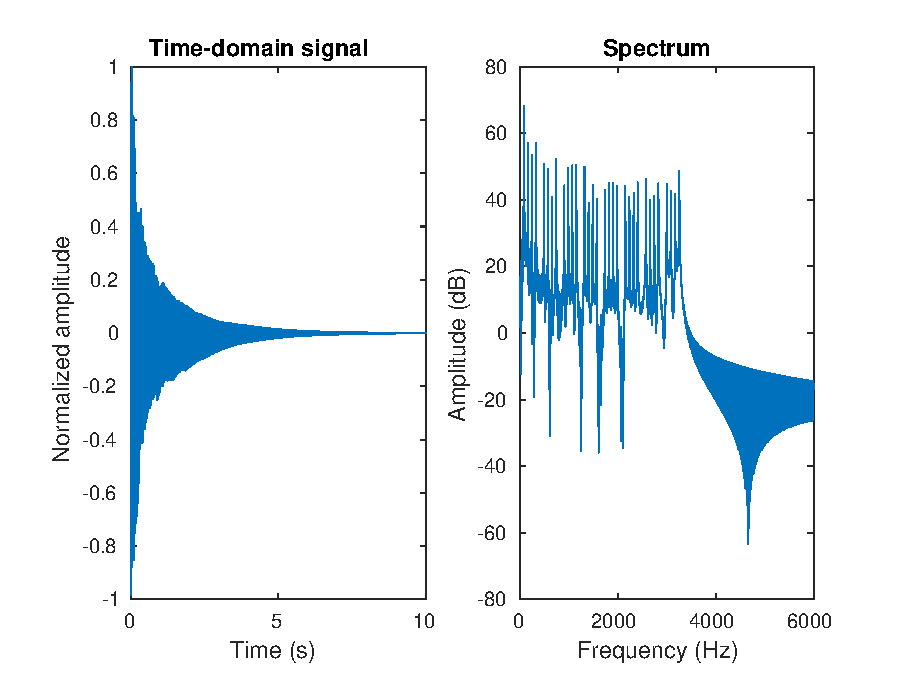
\includegraphics[scale=0.8]{figures/modal_synthesis-E2-40_string_modes-15_body_modes-finger_pluck.eps}
 \caption{Synthèse modale, \( E2 \), largeur de doigt, \( 40 \) modes de corps
 \label{fig:synth:modal_synth}}
\end{table}

% \end{document}
